\section{Evaluation}

We evaluate Meerkat.Graph on single-source context-free path querying scenario.
For evaluation, we use a PC with Ubuntu 18.04 installed.
It has Intel core i7-6700 CPU, 3.4GHz, DDR4 32Gb RAM
The Neo4j database is embedded into the application.

The dataset contains two real-world RDFs: Geospecies which contains information about the biological hierarchy\footnote{Geospecies RDF: \url{https://old.datahub.io/dataset/geospecies}. Access date: 12.03.2020.} and Enzyme which is a part of the UniProt database\footnote{Protein sequences data base: \url{https://www.uniprot.org/}. RDFs with data are avalable here: \url{ftp://ftp.uniprot.org/pub/databases/uniprot/current_release/rdf}. Access date: 12.03.2020.}.
A detailed description of these graphs is presented in table~\ref{tbl:datasetDetails}.
Note, that graphs were loaded into database fully by using Neosemantix tool\footnote{Neosemantix is a Neo4j plugin for RDF to Neo4j import. Project page: \url{https://neo4j.com/labs/nsmtx-rdf/}. Access date: 30.03.2020.}, not only edges labeled by relations used in queries.

{
\setlength{\tabcolsep}{4pt}
\begin{table}[ht]
\begin{tabular}{|c|c|c|c|c|c|c|c|}
\hline
 Graph      & \#V & \#E & \#SCO & \#T & \#NT & \#BT \\
 \hline
 Enzyme     & 15088  & 47953   & 8202 & 15081 & 6819  & 8195 \\
 Geospecies & 225134 & 1631525 & 0    & 89062 & 20830 & 20867 \\
 \hline
\end{tabular}
\caption{Details of graphs}
\label{tbl:datasetDetails}
\end{table}
}

Queries for evaluation are versions of same-generation query~---~classical context-free query which is useful for hierarchy analysis.
All queries in our evaluation created by using functions described in section~\ref{sect:combinators}. Namely, we create and evaluate three queries $Q_1$, $Q_2$ and $Q_3$ as presented below.

\begin{lstlisting}
def q1 (startV) =
    val q =
        sameGen(makeBrs(RDFS__SUB_CLASS_OF ::
                        RDF__TYPE :: Nil))
    queryFromV(startV, q)
\end{lstlisting}

\begin{lstlisting}
def q2 (startV) =
    val q =
        sameGen(makeBrs(SKOS__BROADER_TRANSITIVE :: Nil))
    queryFromV(startV, q)
\end{lstlisting}

\begin{lstlisting}
def q3 (startV) =
    val q =
        sameGen(makeBrs(SKOS__NARROWER_TRANSITIVEY :: Nil))
    queryFromV(startV, q)
\end{lstlisting}

As you can see, once you create a set of appropriate functions, one can easily construct new queries.

For each graph and each query, we run this query form each vertex from graph and measure elapsed time and required memory by using ScalaMeter library\footnote{ScalaMeter library Web page: \url{https://scalameter.github.io/}. Access date: 12.03.2020.}.

Results of evaluation are presented in figures~\ref{fig:time_per_paths_SCO} and~\ref{fig:mem_per_paths_SCO} for query $Q_1$, in figures~\ref{fig:time_per_paths_BT} and~\ref{fig:mem_per_paths_BT} for query $Q_2$, and in figures~\ref{fig:time_per_paths_NT} and~\ref{fig:mem_per_paths_NT} for query $Q_3$. 
Note that some results on time and meoty mesauremnts are presented in Appendix~\ref{sec:evlaDetails}.
For each query result size we calaulate an average value of requred time and memory, and for each set of points we also draw linear approcsimation of this set. While memory consumption is qite stable, time measuremets contain outlayers but they are not sufficient. To demonstarte it we provide standart boxplot for $Q_3$ in figure~\ref{fig:time_per_paths_NT_boxplot}. 
Also we collect paths length distribution which is showed in figure~\ref{fig:pLength}.

\begin{figure}[ht]
  \begin{center}
    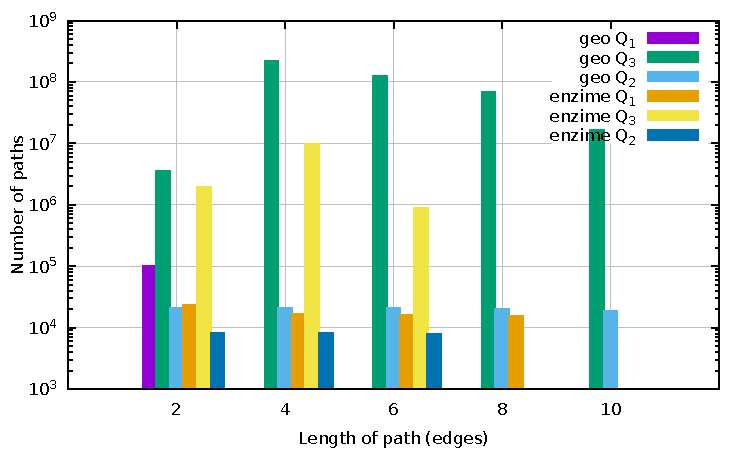
\includegraphics[width=0.5\textwidth]{data/path_per_length.pdf}
    \caption{Paths length distribution}\label{fig:pLength}
  \end{center}
\end{figure}

\begin{figure}[ht]
  \begin{center}
    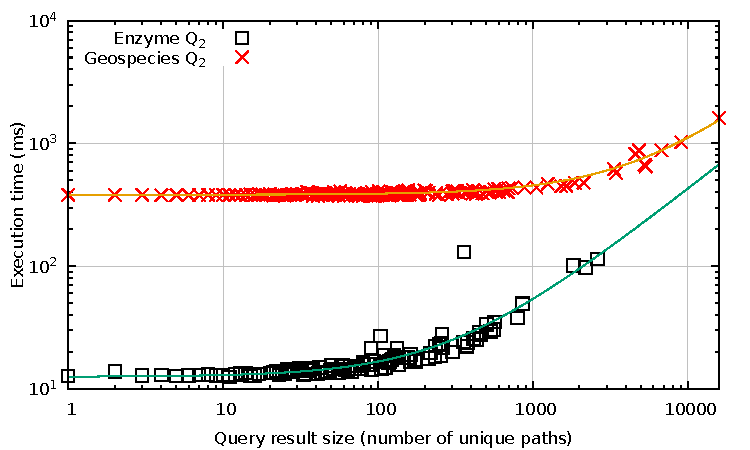
\includegraphics[width=0.5\textwidth]{data/time_per_paths_BT.pdf}
    \caption{Execution time for $Q_2$ query}
    \label{fig:time_per_paths_BT}
  \end{center}
\end{figure}


First of all, we can see that provided datasets contain relatively short paths which satisfy queries: the longest path for all queries contains 10 edges. 

Figures~\ref{fig:time_per_paths_BT},~\ref{fig:time_per_paths_NT} and~\ref{fig:time_per_paths_SCO} show dependency of query evaluation time on query result size measured in terms of number of unique paths.
First, we can see that query evaluation time is linear on result size. 
Also we can see, that time which requred to evaluate query for one specific vertex is relatively small.
For example, for $Q_2$ and Enzyme RDF 15051 queryes (99.75\%) were executed in less then 20ms, and only 3 quweryes requre more than 100ms. 

\begin{figure}[ht]
  \begin{center}
    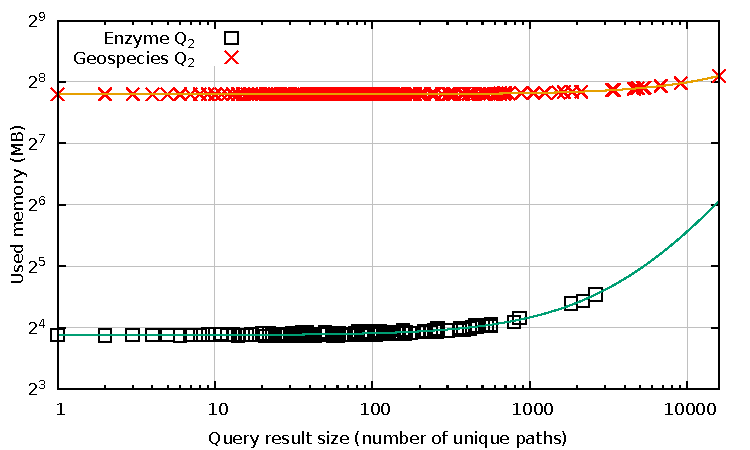
\includegraphics[width=0.5\textwidth]{data/mem_per_paths_BT.pdf}
    \caption{Memory consumption for $Q_2$ query}
    \label{fig:mem_per_paths_BT}
  \end{center}
\end{figure}

Figures~\ref{fig:mem_per_paths_BT},~\ref{fig:mem_per_paths_NT}, and~\ref{fig:mem_per_paths_SCO} show dependency of memory requred to evaluate qurey on query result size. We can see, that memory consumption is linear on result size, and relatively small (not exceed 512 Mb even for big results).

We can see, that both, time and memory consumption depend on input graph size, and it dependency looks like constant overhead which independent from query and query result size. It is because of Meerket.Graph is implemented on top of Neo4j and cannot use internal data structures and create an optimal query execution plan. For example, to find start vertex by predicate specified in the query it performs linear scan over all vertices for each query. It is the reason for the time difference between Enzyme and Geospecies datasets. To prevent such problems, query execution mechanisms should be deeply integrated into the database engine.

Finally, we can conclude that confext-free path querying in single-source scenario can be efficiently evaluated in case when number of paths in answer is big but its length is relatively small, while all pairs scenario is still hard~\cite{10.1145/3335783.3335791}.
Also we can see that while theoretical time and space complexity of CFPQ algoritms at leas cubic, in demonstrated scenario real execution time and required memory is linear.
So, it is necessary to provide detailed time and space complexity analysis of algorithms.